\begin{table*}
\begin{boxedminipage}{\textwidth}
\section*{Relational Data Model}
\begin{description}
\setlength\itemsep{6pt}
\item[Relation] 
All data are represented as \emph{relations}.  A relation can be visualized as a table or a shreadsheet.  
It consists of a \emph{heading} with attribute names and datatypes and a \emph{body} comprising a set of \emph{tuples} with values for each attribute.

\begin{center}
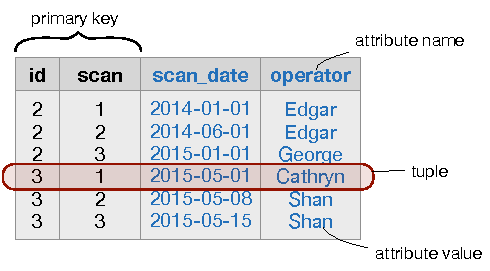
\includegraphics{./figures/relation.pdf}
\end{center}

We distinguish between \emph{base relations} and \emph{derived relations}.  
A base relation has a dedicated class in MATLAB or Python and represents data stored directly in the database.
Derived relations are formed from other relations by using relational operators (See Table \ref{algebra}).
To create a new base relation, users create a new MATLAB or Python class subclassing from the DataJoint Relation class and define the relation's heading. 
After that, users interact with the data by invoking these relation classes.

\item[Schema] A schema is a named collection of related base relations. 
A single project may store data across multiple schemas. Conversely, many schemas can be used for data shared by multiple projects.

\item[Query] Queries retrieve the data represented by a relation into the MATLAB or Python workspace.

\item[Primary key] Every relation has a primary key: a subset of its of attributes that uniquely identify each of its tuples. 
Two tuples with the same values of the primary key attributes cannot coexist in the same relation.
The remaining attributes in the relation are called dependent attributes. 
When one relation includes some attributes that also belong to the primary key of another relation, they determine how tuples are grouped and related between the two relations.

\item[Dependencies]
Base relations may form dependencies by referencing one another. 
Every tuple in a dependent relation must have a matching tuple in the relations references by the dependency. 
Dependencies may cross schema boundaries.

\item[ERD]
The entity relationship diagram or ERD is a graphical representation of base relations and their dependencies.
Fig.\ \ref{schema}\,B depicts the ERD for a particular neuroscience experiment. 
\end{description}
\end{boxedminipage}
\caption{Key concepts of the relational data model as used in DataJoint.}
\label{glossary}
\end{table*}
